\documentclass{beamer}

\mode<presentation> {

\usetheme{Berkeley}


}

%Packages
\usepackage{graphicx} % Allows including images
\usepackage{booktabs} % Allows the use of \toprule, \midrule and \bottomrule in tables
\usepackage{hyperref} 
\usepackage[11pt]{moresize}

%-----------------------------------------------------------------------------------
%	TITLE PAGE
%-----------------------------------------------------------------------------------

\title[@Capacity]{
\includegraphics[width=.85\textwidth]{capacity_logo.png}} % The short title appears at the bottom of every slide, the full title is only on the title page

\author{IE 332 Group 11} % Your name
\institute[IE 332 Group 11] % Your institution as it will appear on the bottom of every slide, may be shorthand to save space
{
Purdue University \\ % Your institution for the title page
}
\date{December 3rd, 2018} % Date, can be changed to a custom date



\begin{document}
\setbeamertemplate{footline}[frame number]
\logo{
\includegraphics[width=.1\textwidth]{capacity_logo.png}} %logo throughout presentation


\begin{frame}
\titlepage % Print the title page as the first slide
\end{frame}

%-----------------------------------------------------------------------------------
%	PRESENTATION SLIDES
%-----------------------------------------------------------------------------------

\section{Introduction} 
\begin{frame}
\frametitle{Meet the Team}

\vspace*{11px}

\includegraphics[width=.22\textwidth]{Alex_Name.png}\quad
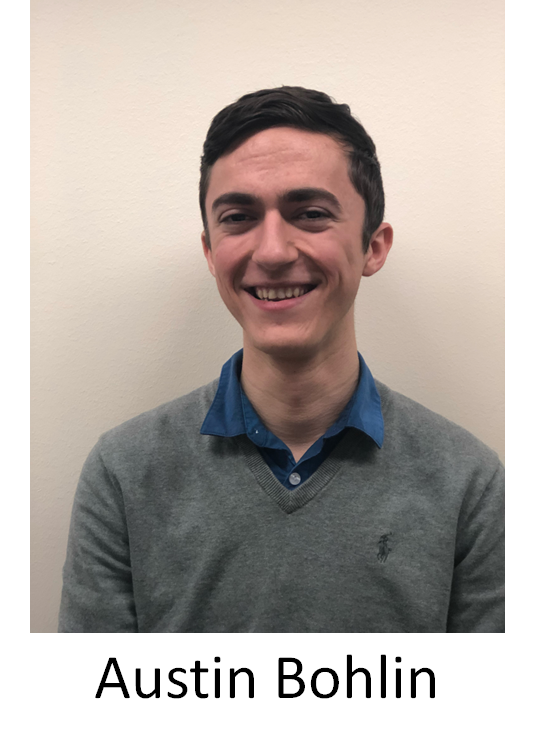
\includegraphics[width=.22\textwidth]{Austin_name.png}\quad
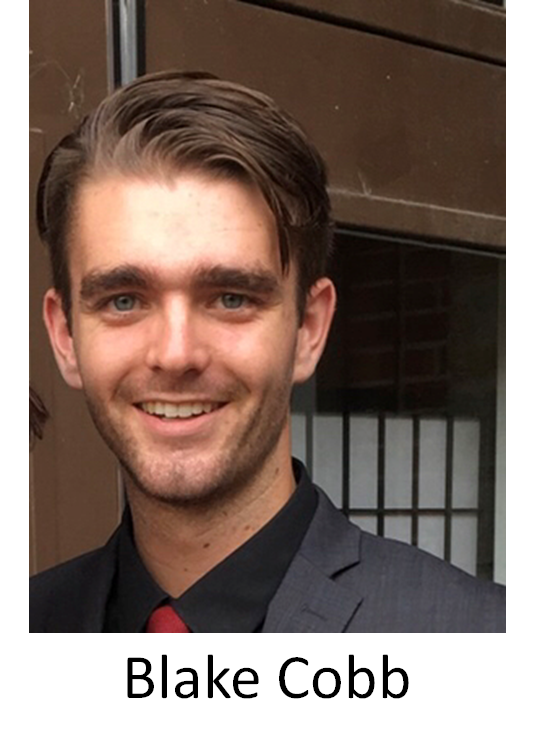
\includegraphics[width=.22\textwidth]{Blake_name.png} \quad
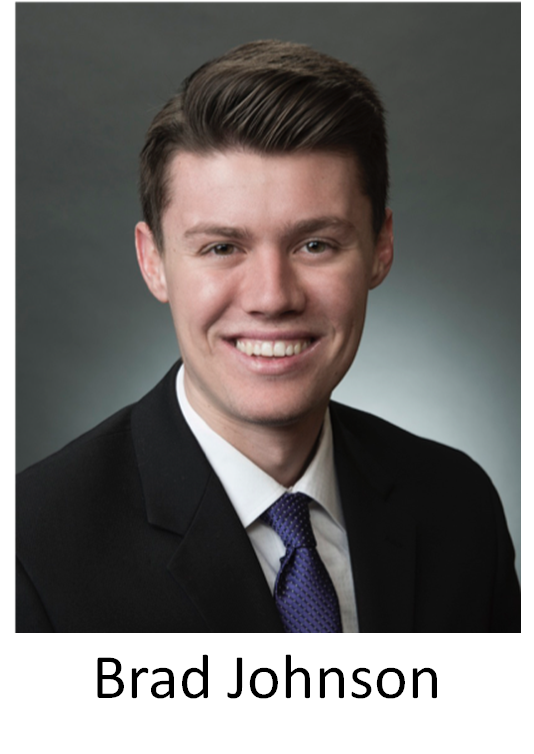
\includegraphics[width=.22\textwidth]{Brad_name.png}\quad
\\[\baselineskip]
\quad\quad
\includegraphics[width=.22\textwidth]{Brandon_Name.png} \quad\quad
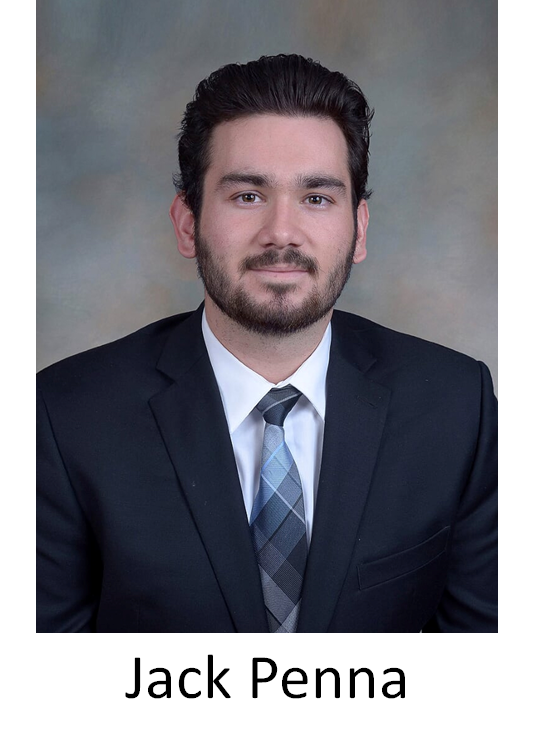
\includegraphics[width=.22\textwidth]{Jack_Name.png}\quad\quad
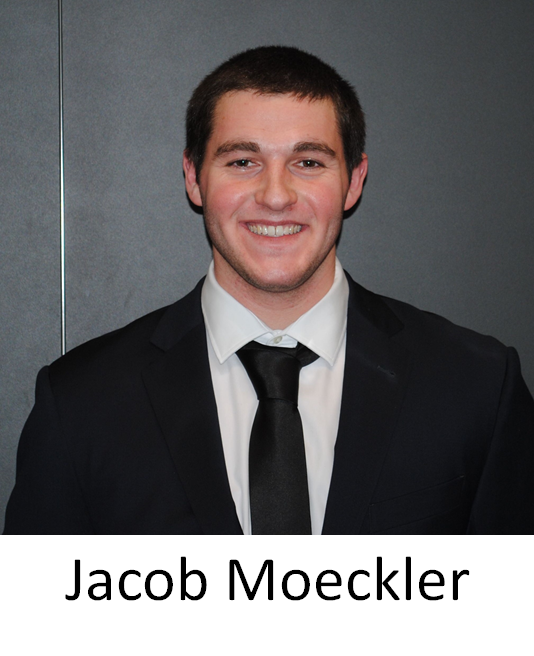
\includegraphics[width=.22\textwidth]{Jacob_Name.png} \quad\quad 


\usebackgroundtemplate{
\includegraphics[width=0.8]{capacity.png}}
%Uncomment the code on this slide to include your own image from the same directory as the template .TeX file.
\begin{figure}

%\includegraphics[width=0.8\linewidth]{frog.jpg}
\end{figure}
\end{frame}


\section{VOC}

\begin{frame}
\frametitle{Voice of the Customer}


% Please add the following required packages to your document preamble:
% \usepackage{graphicx}
\begin{table}[]
\centering
\resizebox{\textwidth}{!}{%
\begin{tabular}{|c|c|}
\hline
\textbf{Warehouse Owners} & \textbf{Lessees} \\ \hline
Underutilized warehouses & Difficult to find storage space for unique requirements \\ \hline
Difficult to manage multiple warehouses & Tedious process to determine warehouse details \\ \hline
Finding 1:1 Relationships with Lessees &  \\ \hline
Maintenance Issues &  \\ \hline
\end{tabular}%
}
\end{table}


\textbf{GOAL:} Provide warehouse owners and potential lessees a platform to efficiently search for and form 1:1 relationships that minimizes underutilized space and maximize customer satisfaction. \\


\textbf{SOLUTION: }@Capacity is a peer-to-peer warehouses sharing company that allows customers to find warehouses and lessees via our website. \\
% Address these aforementioned problems while providing warehouse owners and potential lessees with a unique solution that provides efficient collaboration to minimize underutilized space and maximize customer satisfaction.
\end{frame}

% \begin{frame}
% \frametitle{@Capacity Solutions}
% \textbf{SOLUTION: }@Capacity is a peer-to-peer warehouses sharing company that allows customers to find warehouses and lessees via our website. \\


%  \fbox{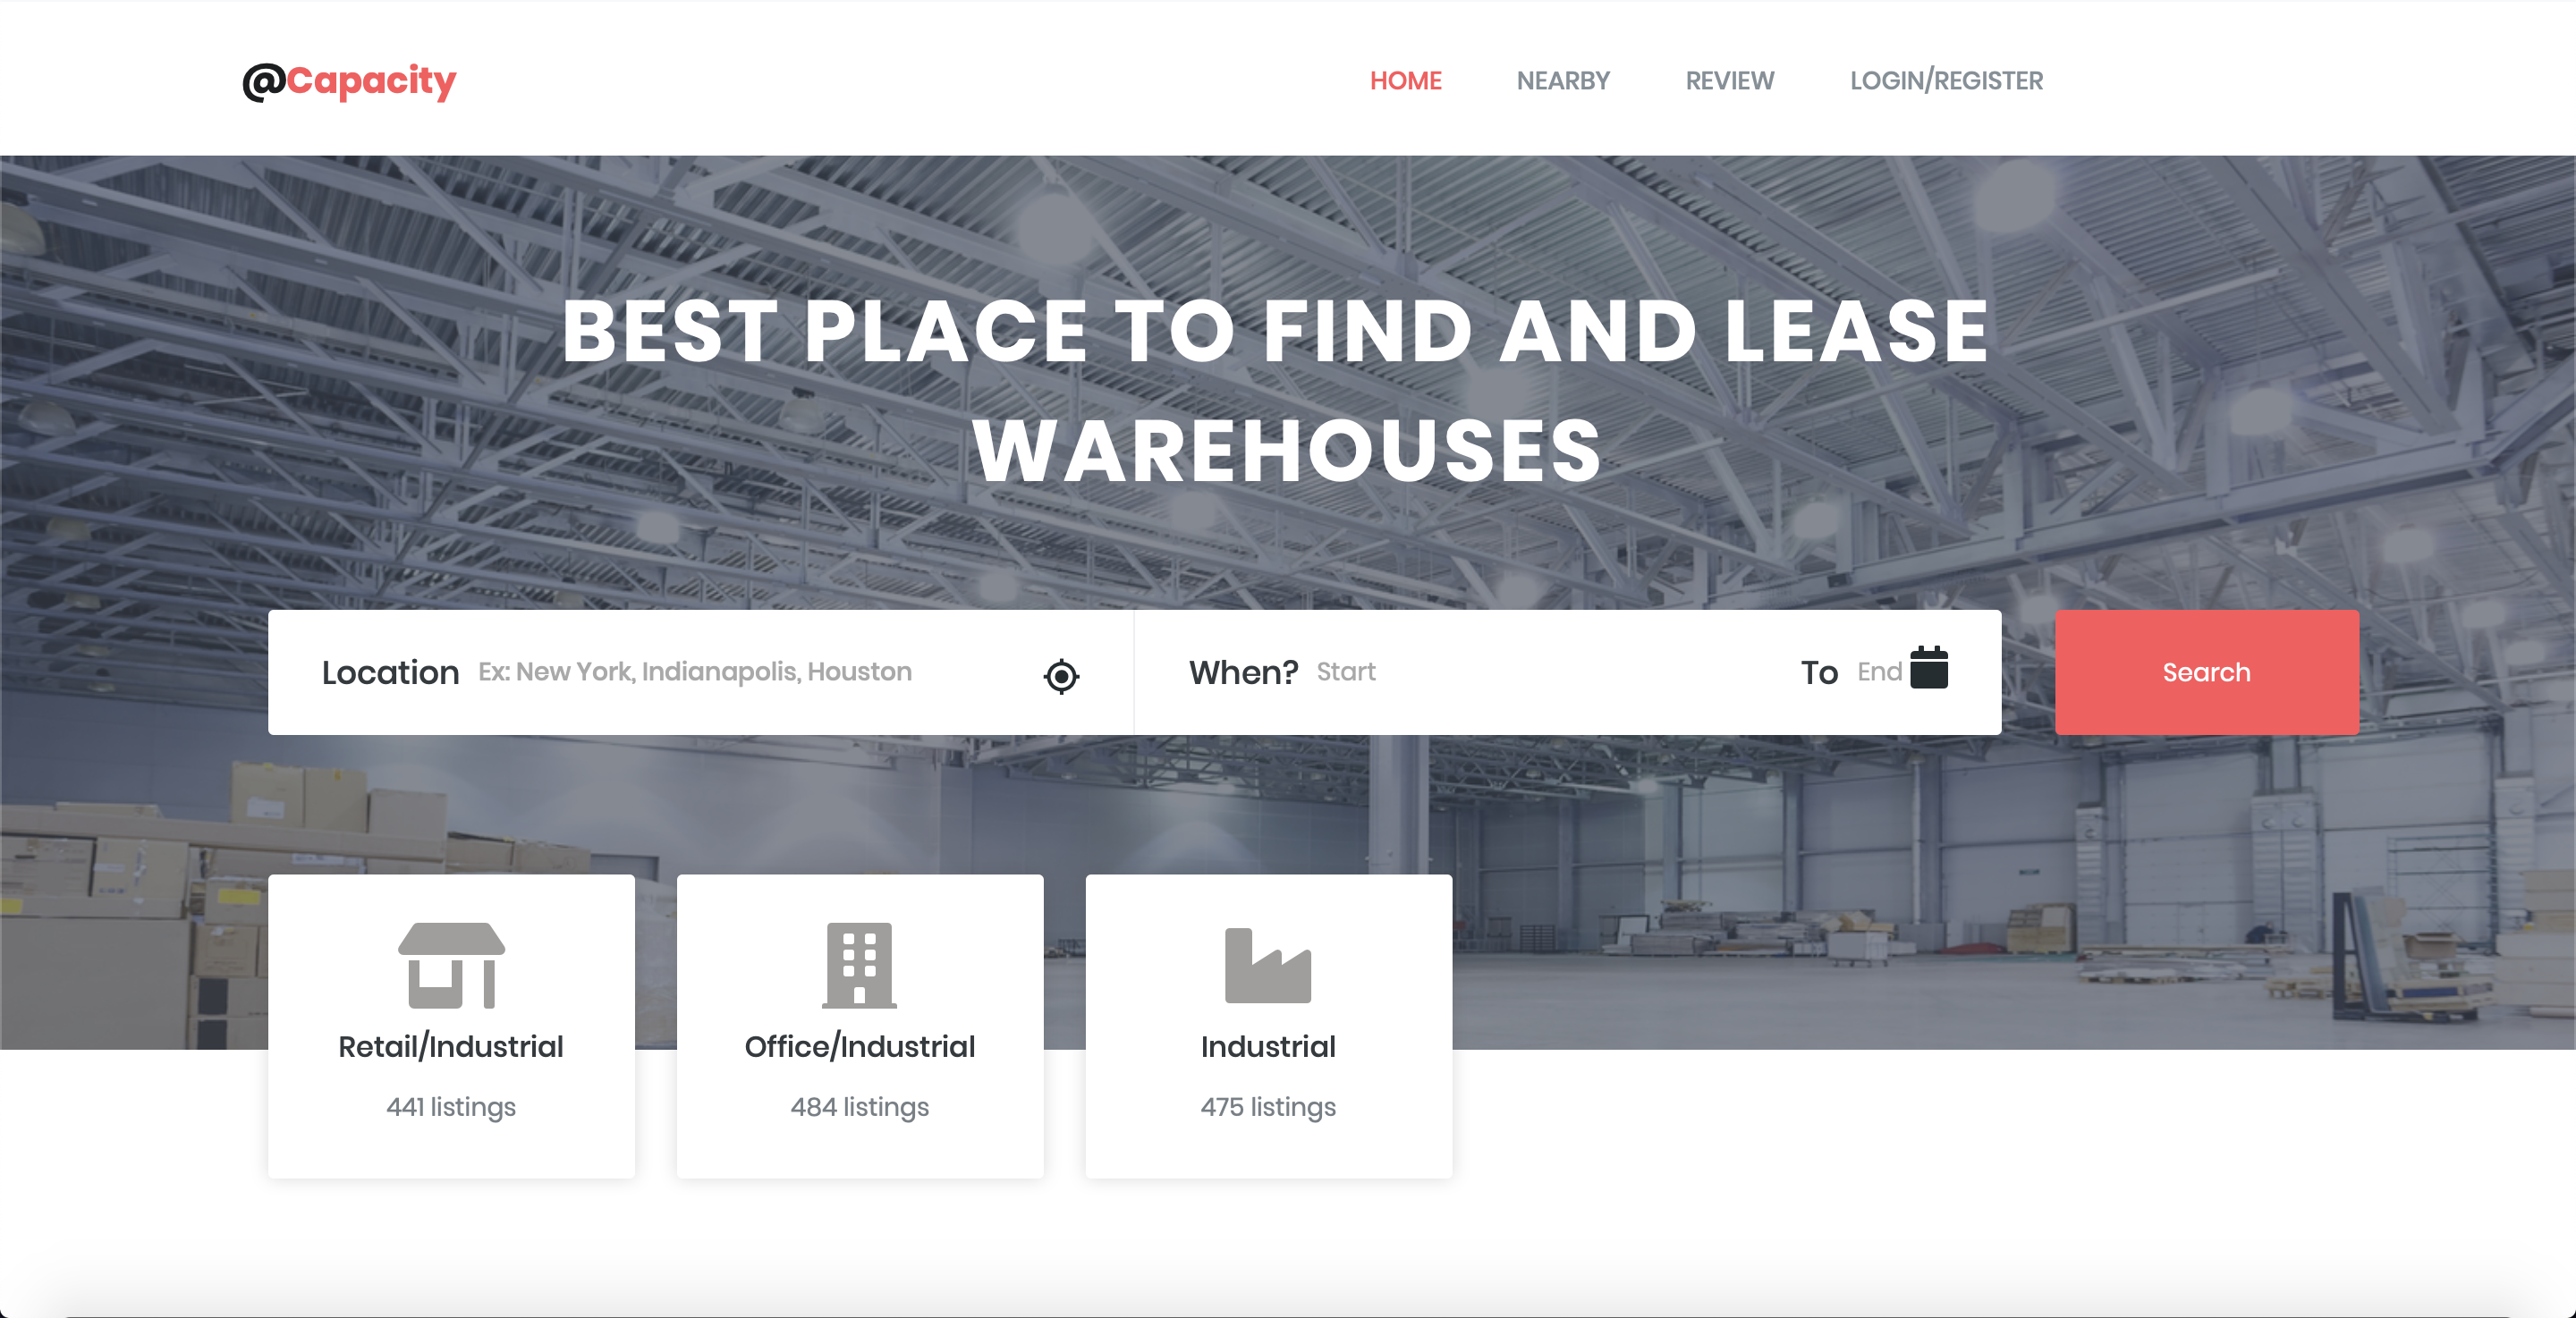
\includegraphics[width=\textwidth]{Homepg.png}}

% \end{frame}


\section{@Capacity Solution}


\begin{frame}
\frametitle{@Capacity Solutions} \footnotesize
\begin{block}{Flexibility}
\begin{itemize}
\item Lessees get customized list of warehouses based on their situation.
\item Owners have the power to accept or deny a proposed contract by the lessee. 
\end{itemize}
% Lessees have the power to choose warehouses from a personalized list based on user preferences. Owners have the power to accept or deny a proposed contract by the lessee.
\end{block}
\begin{block}{Quality Control}
\begin{itemize}
\item Warehouse Owners can rate Lessee's based on verified previous contract
\item Lessee's can rate the spaces and owners of a previous contract
\end{itemize}
\end{block}
\begin{block}{Intuitive and Informative Interface}
\begin{itemize}
\item Easy for Owners and Lessees to register on our website, as well as to keep track of shipments, pricing, and partner satisfaction.
\end{itemize}
\end{block}
\end{frame}

\subsection{Utilization}

%\begin{frame}
%\frametitle{@Capacity Solutions}
%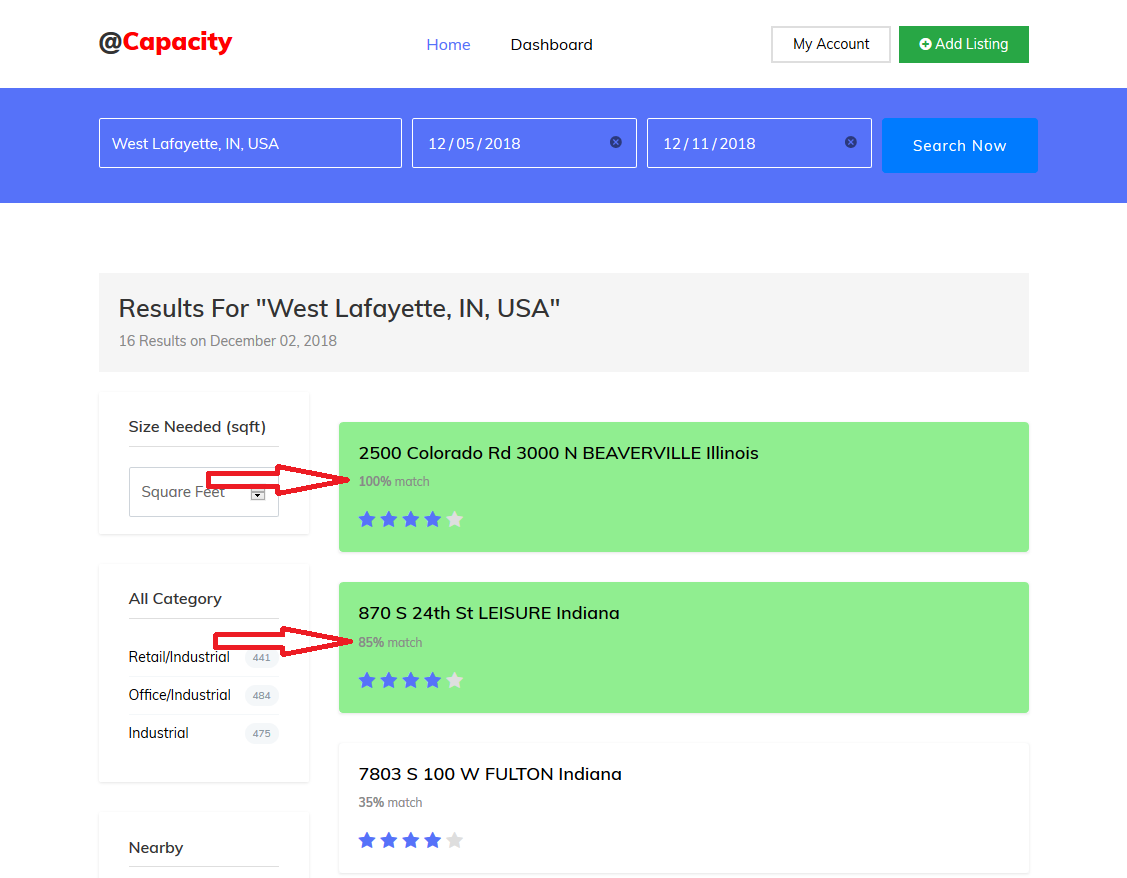
\includegraphics[keepaspectratio=true,width=.8\paperwidth]{utilization.png}

%\begin{columns}[c] % The "c" option specifies centered vertical alignment while the "t" option is used for top vertical alignment
%\begin{column}{.4\linewidth}
%\textbf{Utilization: }Underutilized warehouses are listed closer to the top of the search list page
%\end{column}
%\begin{column}{.6\linewidth}
%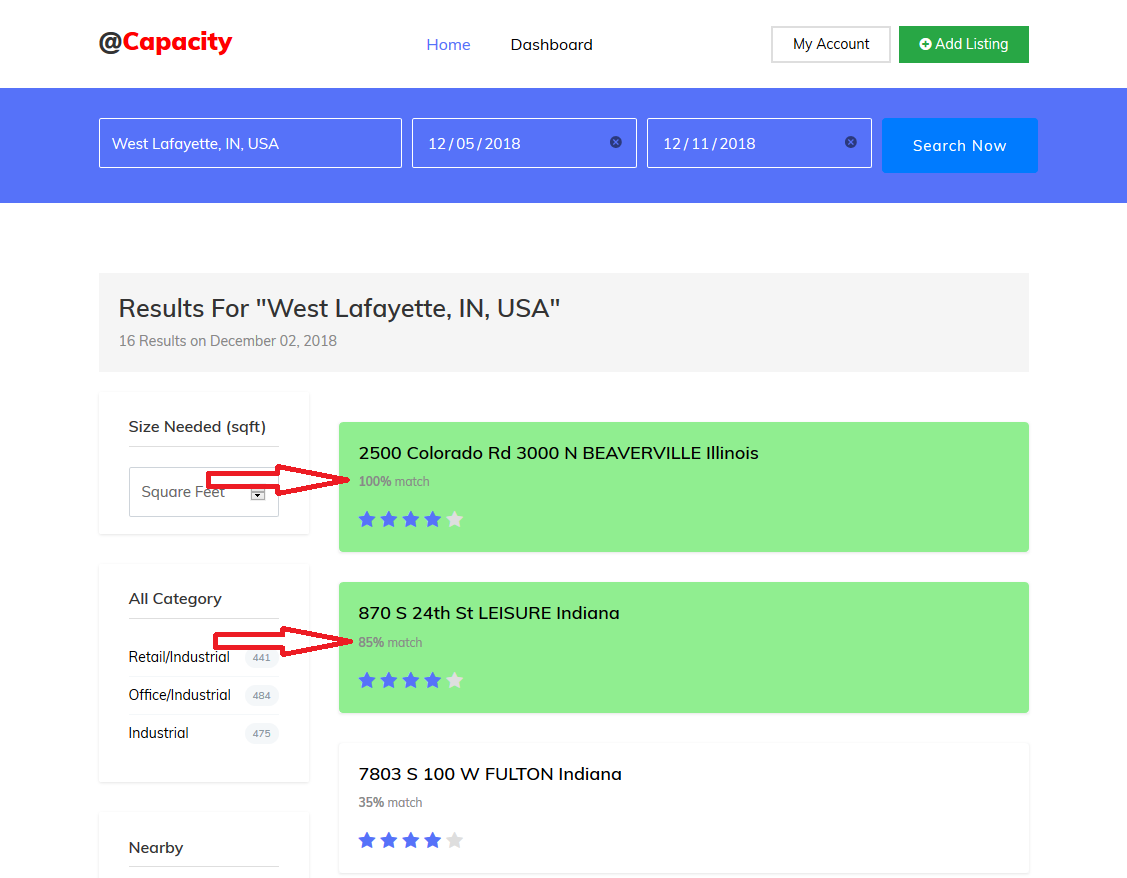
\includegraphics[width=\linewidth]{utilization}
%\end{column}
%\end{columns}
%\end{frame}

\begin{frame}
\frametitle{@Capacity Solutions: Utilization}
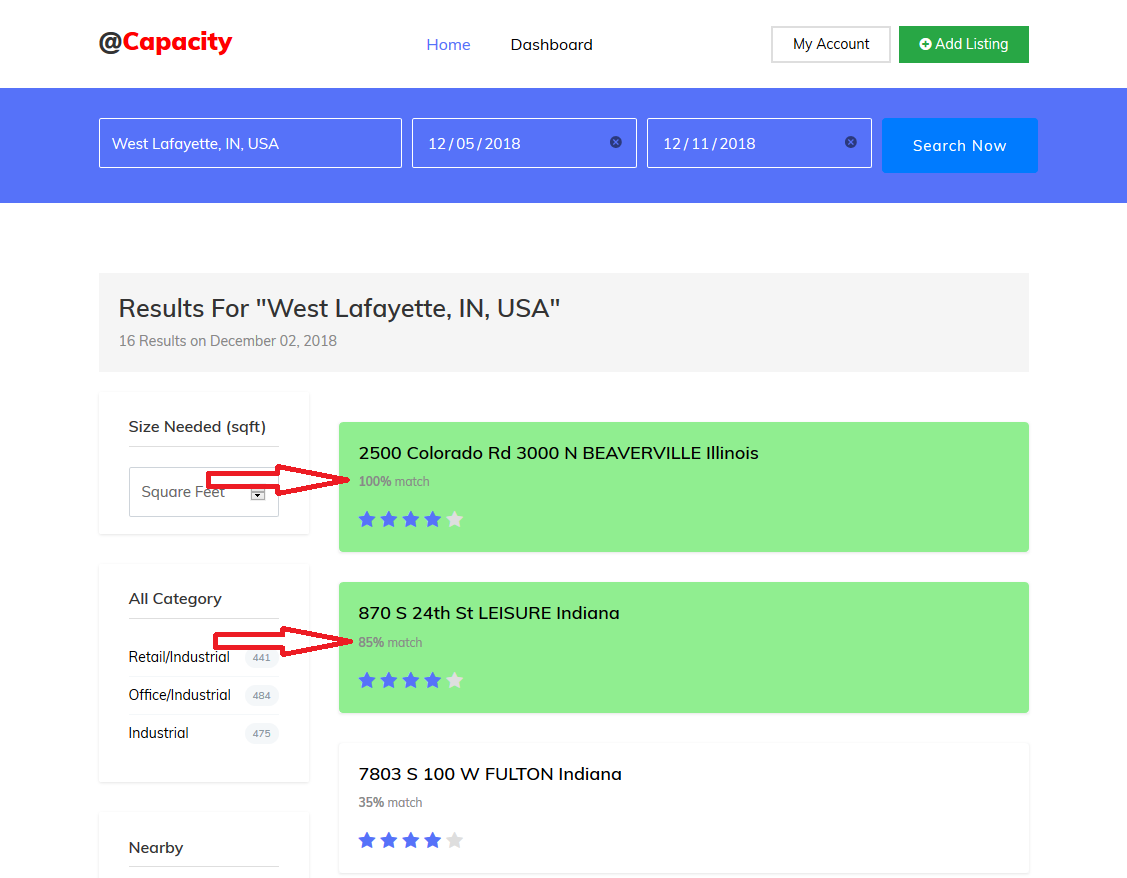
\includegraphics[keepaspectratio=true,width=.8\paperwidth]{utilization.png}
\end{frame}


\subsection{@Capacity Solutions: Reward-Based Discount}

\begin{frame}
\frametitle{@Capacity Solutions: Rewards}
\begin{columns}[c] % The "c" option specifies centered vertical alignment while the "t" option is used for top vertical alignment

\column{.35\textwidth} % Left column and width
\textbf{Reward-Based Discount for Owners: } Owners are incentivized to reached an annual goal of warehouses leased out per year. 
\column{.6\textwidth} % Right column and width
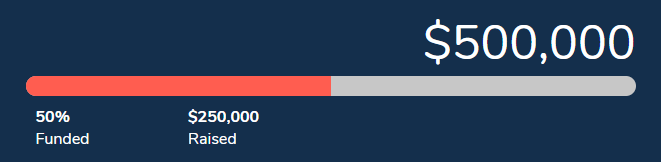
\includegraphics[keepaspectratio=true,width=.5\paperwidth]{thermometer.png}\\
\begin{center} 
Thermometer
\end{center}
\end{columns}
\end{frame}

% \subsection{@Capacity Solutions: Owner Freedom}

% \begin{frame}
% \frametitle{@Capacity Solutions: Owner Freedom}
% \begin{columns}[c] % The "c" option specifies centered vertical alignment while the "t" option is used for top vertical alignment

% \column{.45\textwidth} % Left column and width
% \textbf{Owner Freedom: } Owners can also lease warehouses from their owner account without having to make a new login. 

% \column{.5\textwidth} % Right column and width


% \end{columns}
% \end{frame}


\section{Financial Impact}

\begin{frame}
\frametitle{Financial Impact}
\textbf{Investor Information: }  
\begin{itemize}
\item\textit{Low startup cost:} minimal investment risk 
\item\textit{Self-sustainment:} website with little maintenance and additional capital needed 
\item\textit{Continuous ROI:} 5\% commission on contracts 

\end{itemize}
\end{frame}

% \begin{frame}
% \frametitle{Example}
% \begin{table}[tp]
% % \centering
% \begin{tabular}{l l l}
% % \vline
% \toprule
% \textbf{Area} & \textbf{Warehouse Type} & \textbf{Amenities}\\
% \midrule
% Missoula, Montana & Industrial & Bay Doors \\
% \bottomrule
% \end{tabular}
% \caption{Lessee wants/needs}

% \includemovie{1cm}{1cm}{fin.gif}

% \end{table}
% \end{frame}

\section{Example}

% \begin{frame}
% \frametitle{Example}
% \begin{columns}[c]
% \column{.45\textwidth} % Left column and width
% \begin{table}[]
% \begin{tabular}{|c|c|}
% \hline
% \textbf{Area}           & Missoula, Montana \\ \hline
% \textbf{Warehouse Type} & Industrial        \\ \hline
% \textbf{Amenities}      & Bay Doors         \\ \hline
% \end{tabular}
% \end{table}
% \end{columns}
% \end{frame}

\begin{frame}
\frametitle{Example}
\begin{columns}[c]
\column{.4\textwidth}
\textbf{Lessee Needs: } 
\begin{itemize}
\item\textit{Area}: Missoula, MT
\item\textit{Building Type}: Industrial
\item\textit{Amenities}: Bay Doors
\end{itemize}
\column{.65\textwidth} % Right column and width
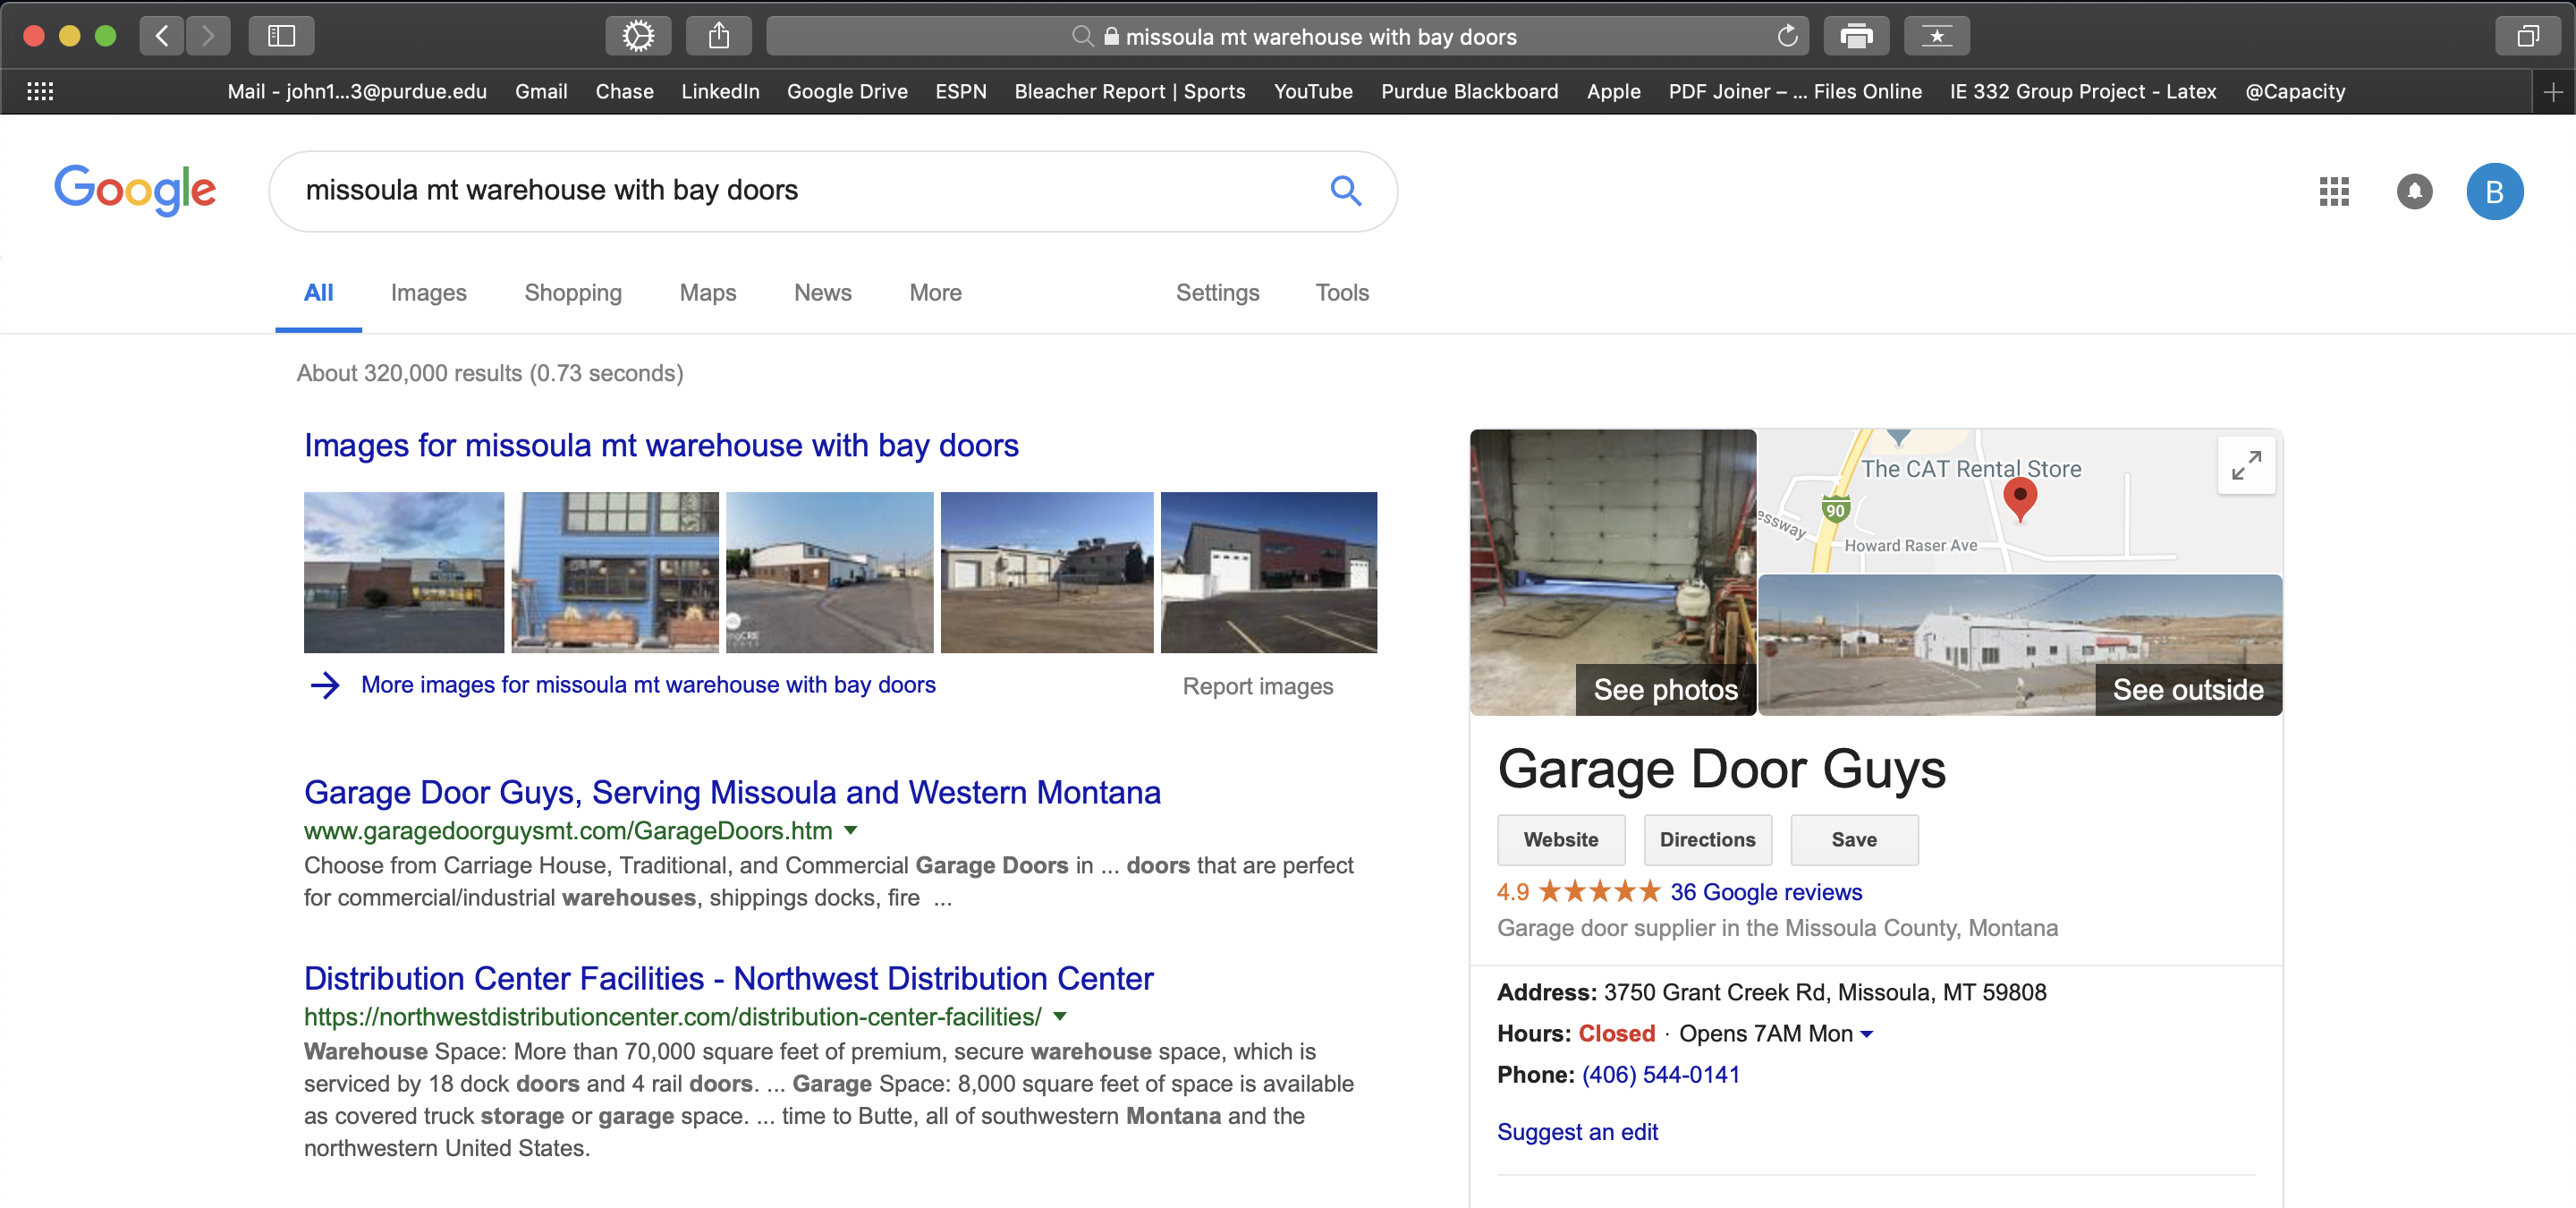
\includegraphics[width=1\textwidth]{Screenshot.png}
\end{columns}
\end{frame}


\begin{frame}
\frametitle{Example (Cont.)}
\begin{columns}[c]
\column{.4\textwidth}
\textbf{Lessee Needs: } 
\begin{itemize}
\item\textit{Area}: Missoula, MT
\item\textit{Building Type}: Industrial
\item\textit{Amenities}: Bay Doors
\end{itemize}
\column{.65\textwidth} % Right column and width
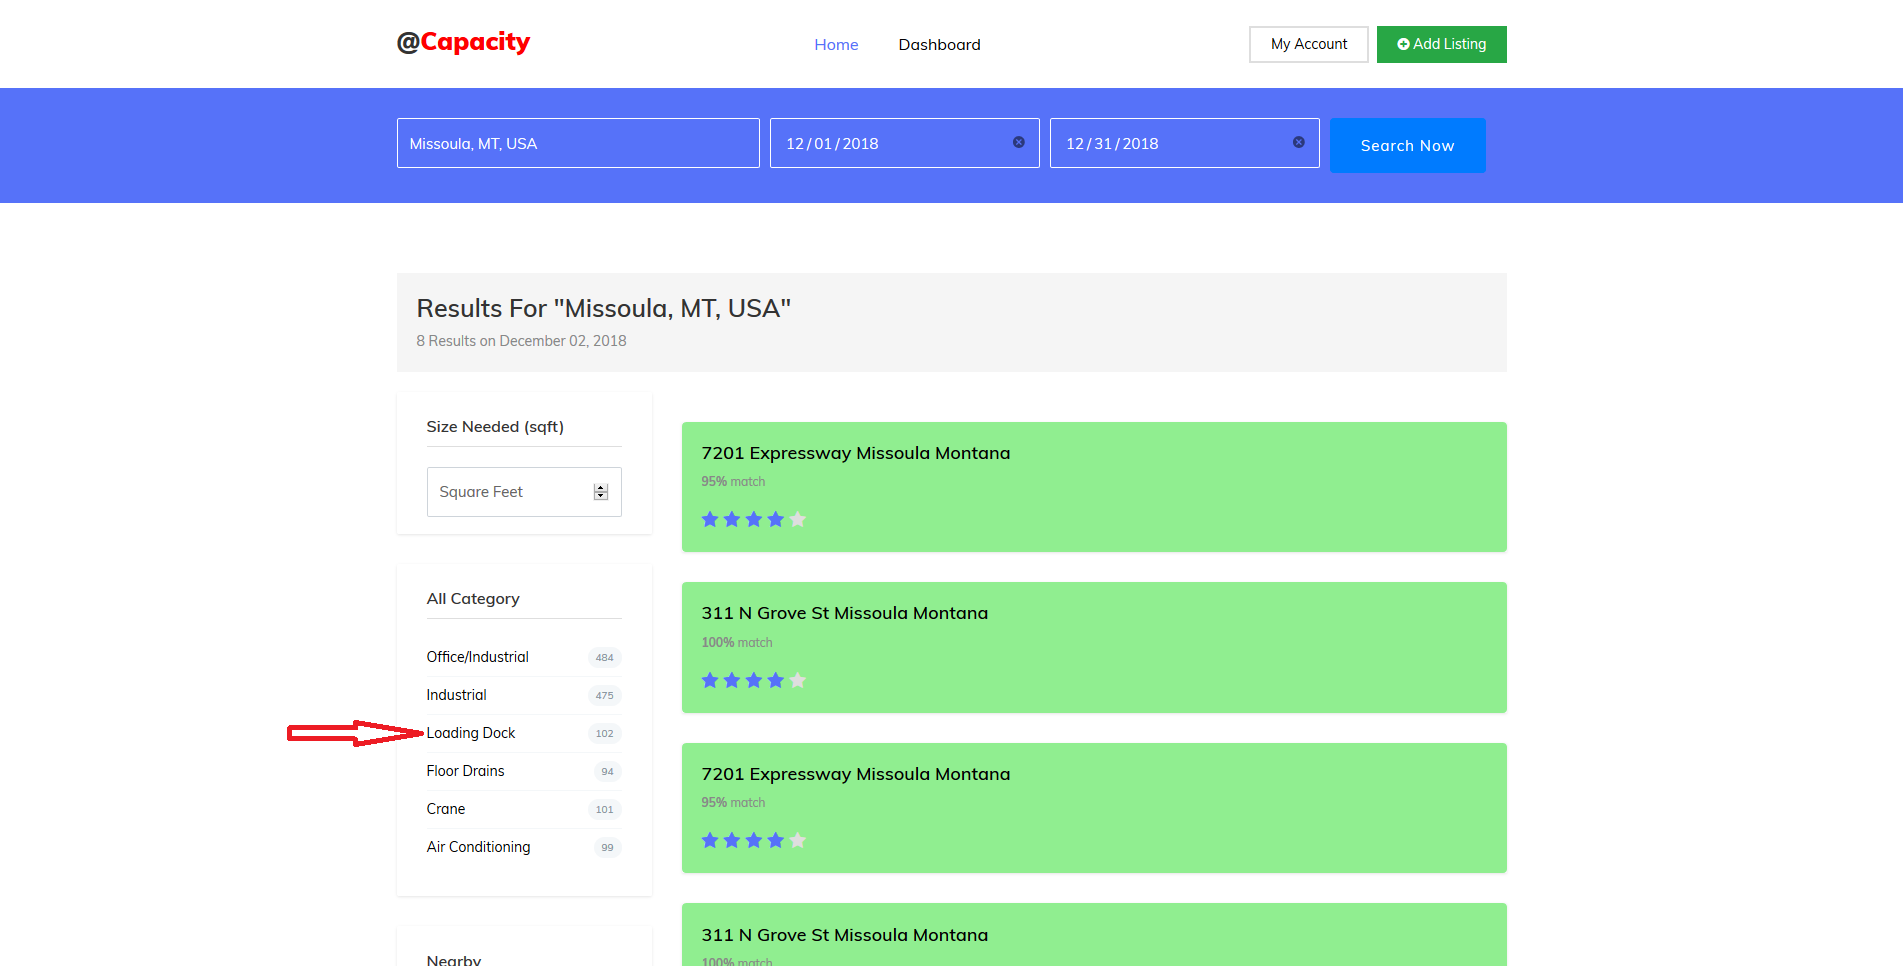
\includegraphics[width=1\textwidth]{loading.png}
\end{columns}
\end{frame}



\section{Conclusion}

\begin{frame}
\frametitle{Thank you!}

\begin{center}

\vspace*{7px}

\includegraphics[width=.2\linewidth]{facebook.png}\quad \href{https://www.facebook.com/AtCapacity-339587599924715/}{Facebook: atCapacity}
\\[\baselineskip]% adds vertical line spacing

\includegraphics[width=.2\linewidth]{insta.jpg}\quad \href{ https://www.instagram.com/capacity332/}{Instagram: capacity332}
\\[\baselineskip]

\includegraphics[width=.2\linewidth]{twitter.png}\quad \href{https://twitter.com/Capacity_332}{Twitter: Capacity\underline{\hspace{5px}}332}
\end{center}
\end{frame}



\end{document} 